\documentclass[aspectratio=169,11pt]{beamer}

\usetheme{Madrid}
\usecolortheme{default}
\setbeamertemplate{navigation symbols}{}
\setbeamertemplate{footline}[frame number]

\usepackage{amsmath,amssymb,booktabs}
\usepackage{graphicx}

\graphicspath{{assets/}}
\pdfstringdefDisableCommands{\def\translate#1{#1}}

\definecolor{UofTBlue}{RGB}{0,45,114}
\definecolor{SoftBlue}{RGB}{233,240,252}
\definecolor{SoftRed}{RGB}{252,237,237}
\definecolor{SoftGreen}{RGB}{230,248,230}
\setbeamercolor{structure}{fg=UofTBlue}
\setbeamercolor{palette primary}{bg=UofTBlue!85!black,fg=white}
\setbeamercolor{palette tertiary}{bg=UofTBlue,fg=white}
\setbeamercolor{frametitle}{fg=UofTBlue,bg=SoftBlue}
\setbeamercolor{block title}{fg=UofTBlue,bg=SoftBlue}
\setbeamercolor{block body}{bg=white}
\setbeamercolor{alertblock title}{fg=black,bg=SoftRed}
\setbeamercolor{alertblock body}{bg=white}

\newenvironment{greenblock}[1]{%
  \setbeamercolor{block title}{fg=black,bg=SoftGreen}%
  \begin{block}{#1}}{\end{block}}

\title[Rage-Bait Lifecycles]{Content-Centric Modelling of Rage-Bait\\
Lifecycles on Social Media with Toxicity Feedback}
\subtitle{APM348 | 10-Minute Presentation}
\author{Neel Sarkar \and Piper Scott Rios}
\institute{University of Toronto}
\date{April 1, 2026}

\begin{document}

% ═══════════════════════════════════════════════════════════════
%  SLIDE 1: TITLE
% ═══════════════════════════════════════════════════════════════
\begin{frame}
  \titlepage
\end{frame}

% ═══════════════════════════════════════════════════════════════
%  SLIDE 2: MOTIVATION
% ═══════════════════════════════════════════════════════════════
\begin{frame}{Why This Matters}
  Engagement-optimized algorithms amplify provocative content.
  This boosts short-term engagement but increases toxicity and
  drives users away \textit{(Brady et al.\ 2017; Beknazar-Yuzbashev et al.\ 2025)}.

  \vspace{0.8em}
  \begin{block}{Central question}
    How does platform amplification shape the full lifecycle of rage-bait,
    and what are the costs for toxicity and user retention?
  \end{block}

  \vspace{0.8em}
  \textbf{Three things we will show:}
  \begin{enumerate}
    \item A sharp amplification \textbf{threshold} exists
    \item Above it, a \textbf{toxicity feedback loop} locks in
    \item The engagement--health \textbf{tradeoff is quantifiable}
  \end{enumerate}
\end{frame}

% ═══════════════════════════════════════════════════════════════
%  SLIDE 3: THE MODEL
% ═══════════════════════════════════════════════════════════════
\begin{frame}{The IVFS Model}
  \begin{columns}[T]
    \begin{column}{0.42\textwidth}
      Six state variables:
      \begin{itemize}
        \item $I, V, F, S$: content lifecycle\\
              {\small ignored $\to$ viral $\to$ fatigued / suppressed}
        \item $\tau$: latent discussion pressure
        \item $U$: active user pool
      \end{itemize}

      \vspace{0.5em}
      \textbf{Key idea:} we classify \emph{content}, not users.
      Platforms rank content; content volumes are directly observable.
    \end{column}
    \begin{column}{0.56\textwidth}
      \centering
      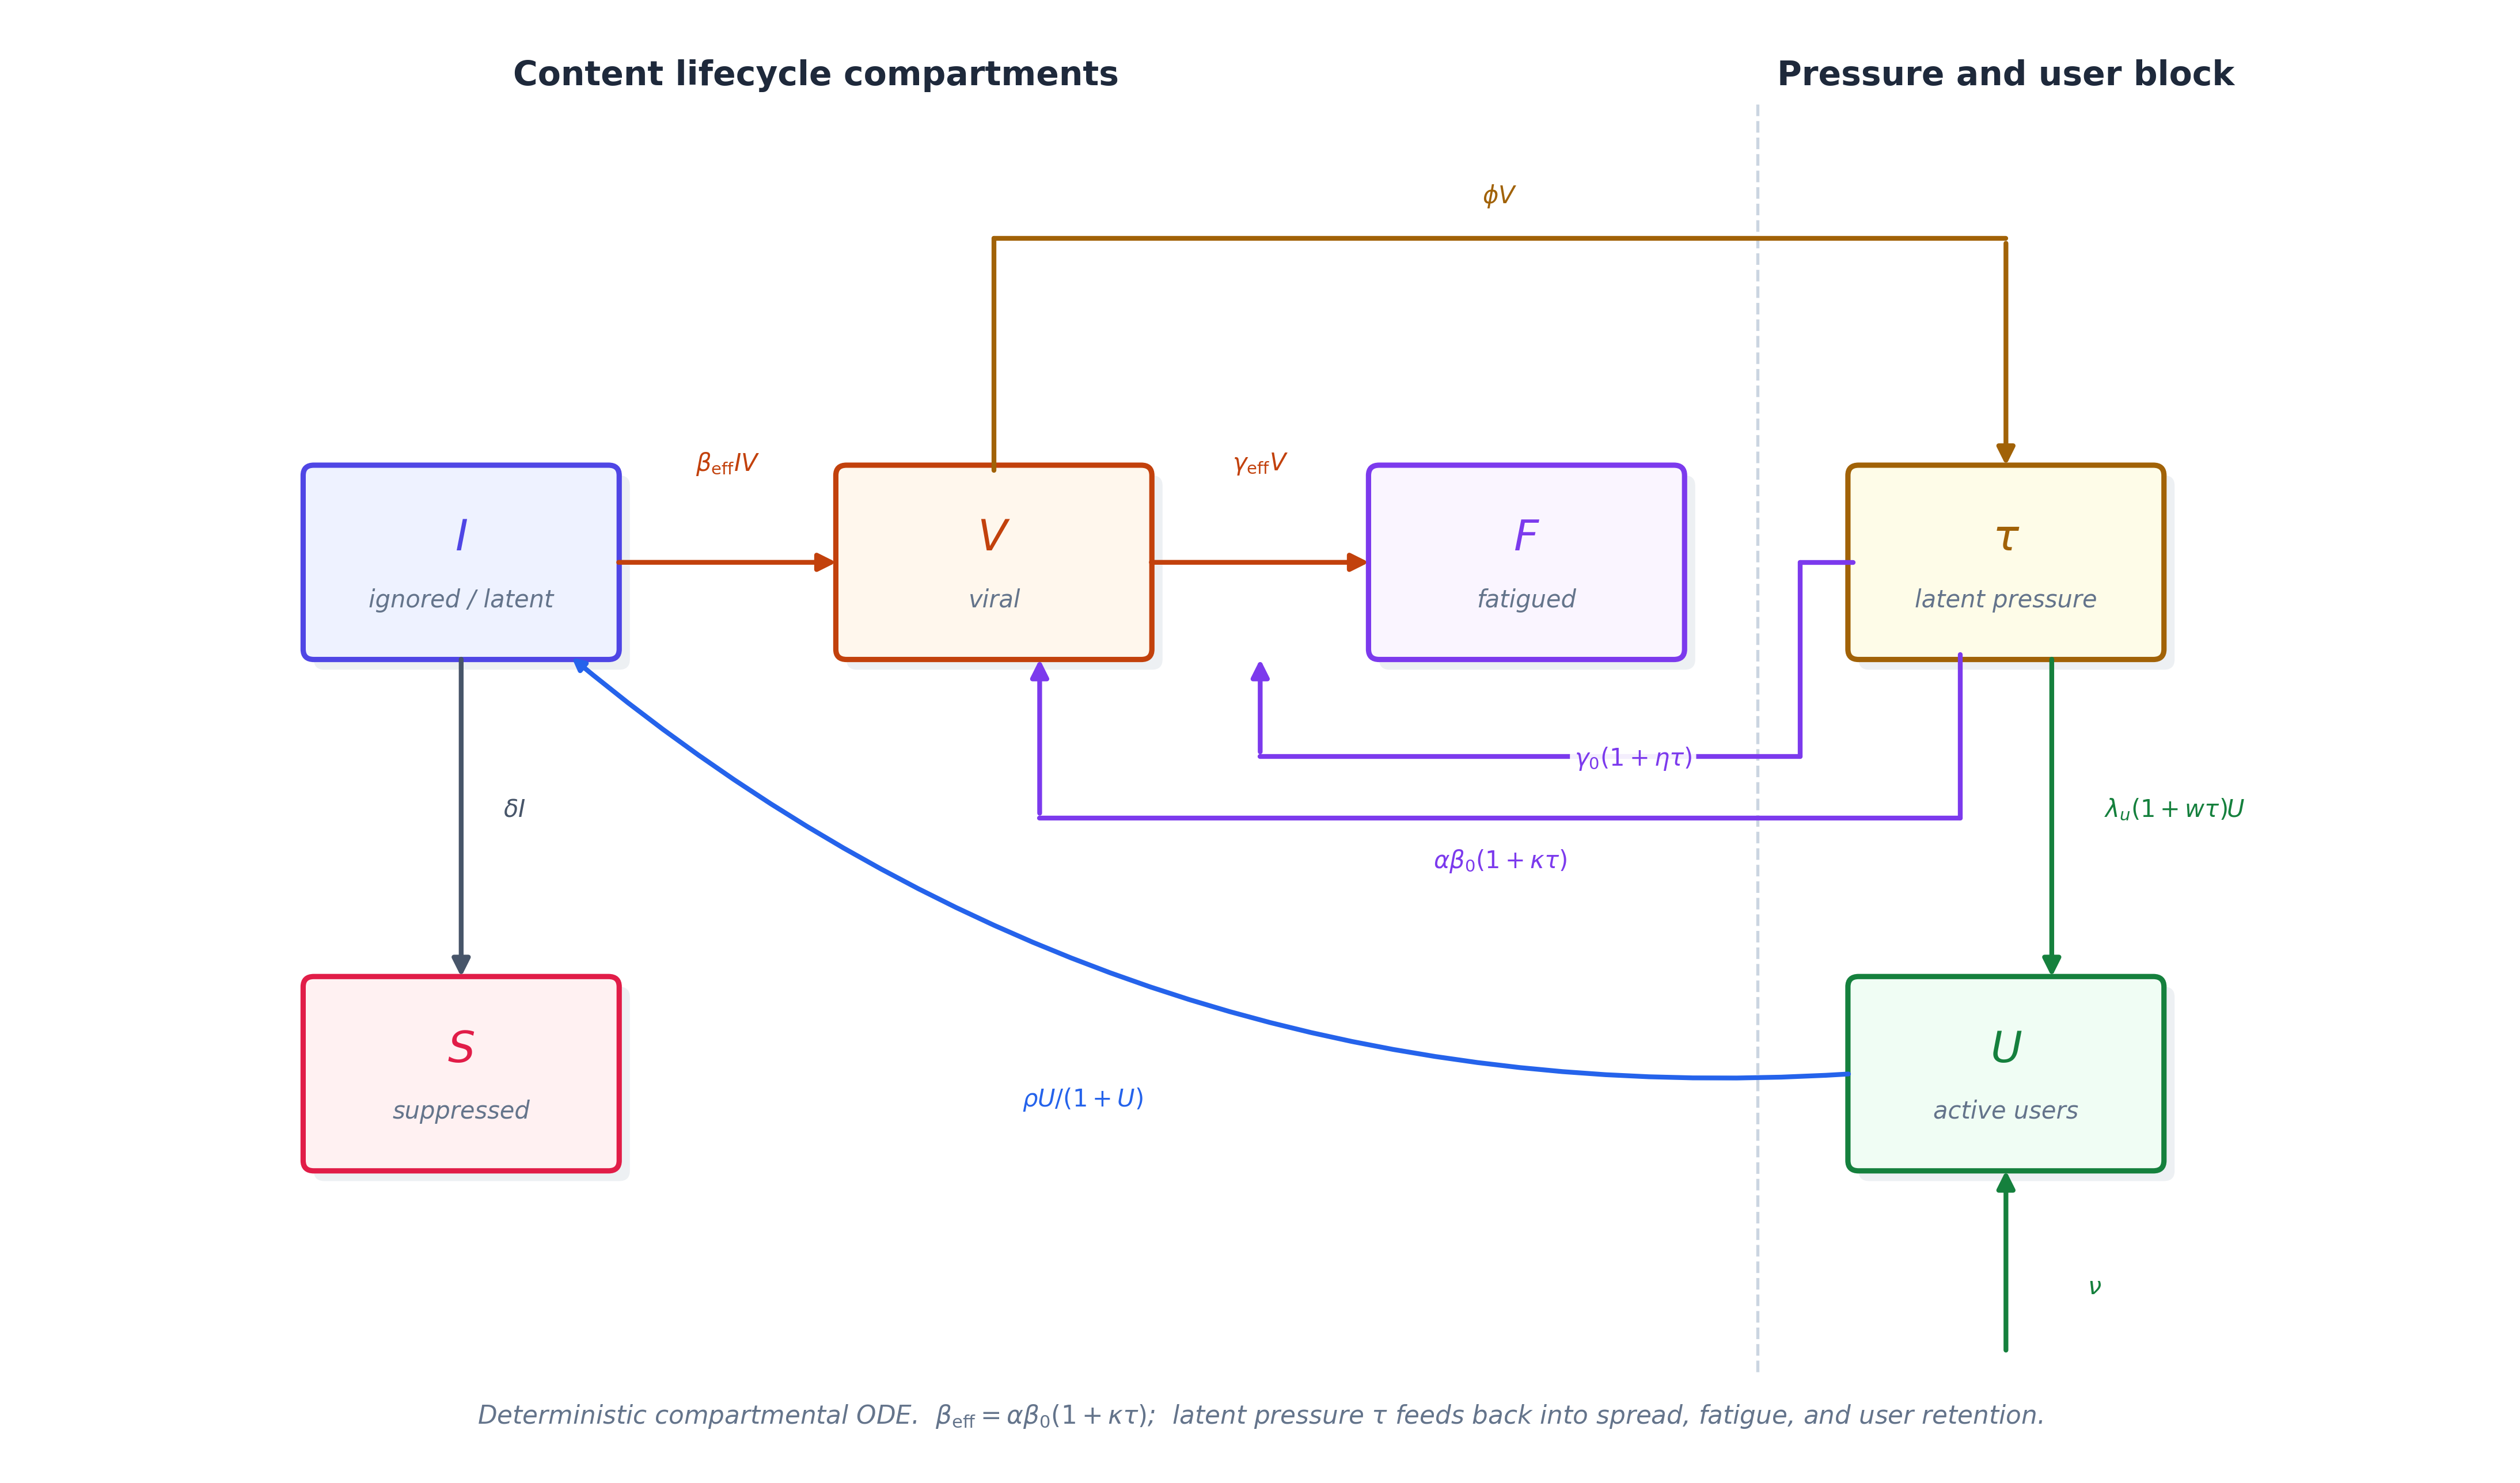
\includegraphics[width=\linewidth,height=0.75\textheight,keepaspectratio]{ivfs_structure_diagram.png}
    \end{column}
  \end{columns}
\end{frame}

% ═══════════════════════════════════════════════════════════════
%  SLIDE 4: THRESHOLD AND FEEDBACK
% ═══════════════════════════════════════════════════════════════
\begin{frame}{Threshold and Feedback Loop}
  \begin{columns}[T]
    \begin{column}{0.50\textwidth}
      \begin{alertblock}{Amplification threshold}
        \[
        \mathcal{R}_0 = \frac{\alpha\,\beta_0\,I_{\mathrm{DFE}}}{\gamma_0 + \mu_c}
        \qquad \boxed{\alpha_{\mathrm{crit}} \approx 0.32}
        \]
      \end{alertblock}

      \vspace{0.4em}
      \begin{itemize}
        \item Below threshold: virality dies out, no pressure
        \item Above threshold: endemic virality, users leave
        \item Transition is \textbf{transcritical}
      \end{itemize}
    \end{column}
    \begin{column}{0.47\textwidth}
      \begin{block}{The toxicity feedback loop}
        \centering
        \vspace{0.2em}
        $V \xrightarrow{\;\phi\;} \tau \xrightarrow{\;\kappa\;} \beta_{\mathrm{eff}} \xrightarrow{} V$
        \vspace{0.2em}
      \end{block}

      \vspace{0.4em}
      Viral content generates discussion pressure,
      which amplifies spread, which creates more viral content.

      \vspace{0.3em}
      Counteracted by fatigue, pressure decay, and user departure.
    \end{column}
  \end{columns}
\end{frame}

% ═══════════════════════════════════════════════════════════════
%  SLIDE 5: RESULTS
% ═══════════════════════════════════════════════════════════════
\begin{frame}{Results: Bifurcation and Policy Tradeoff}
  \begin{columns}[T]
    \begin{column}{0.55\textwidth}
      \centering
      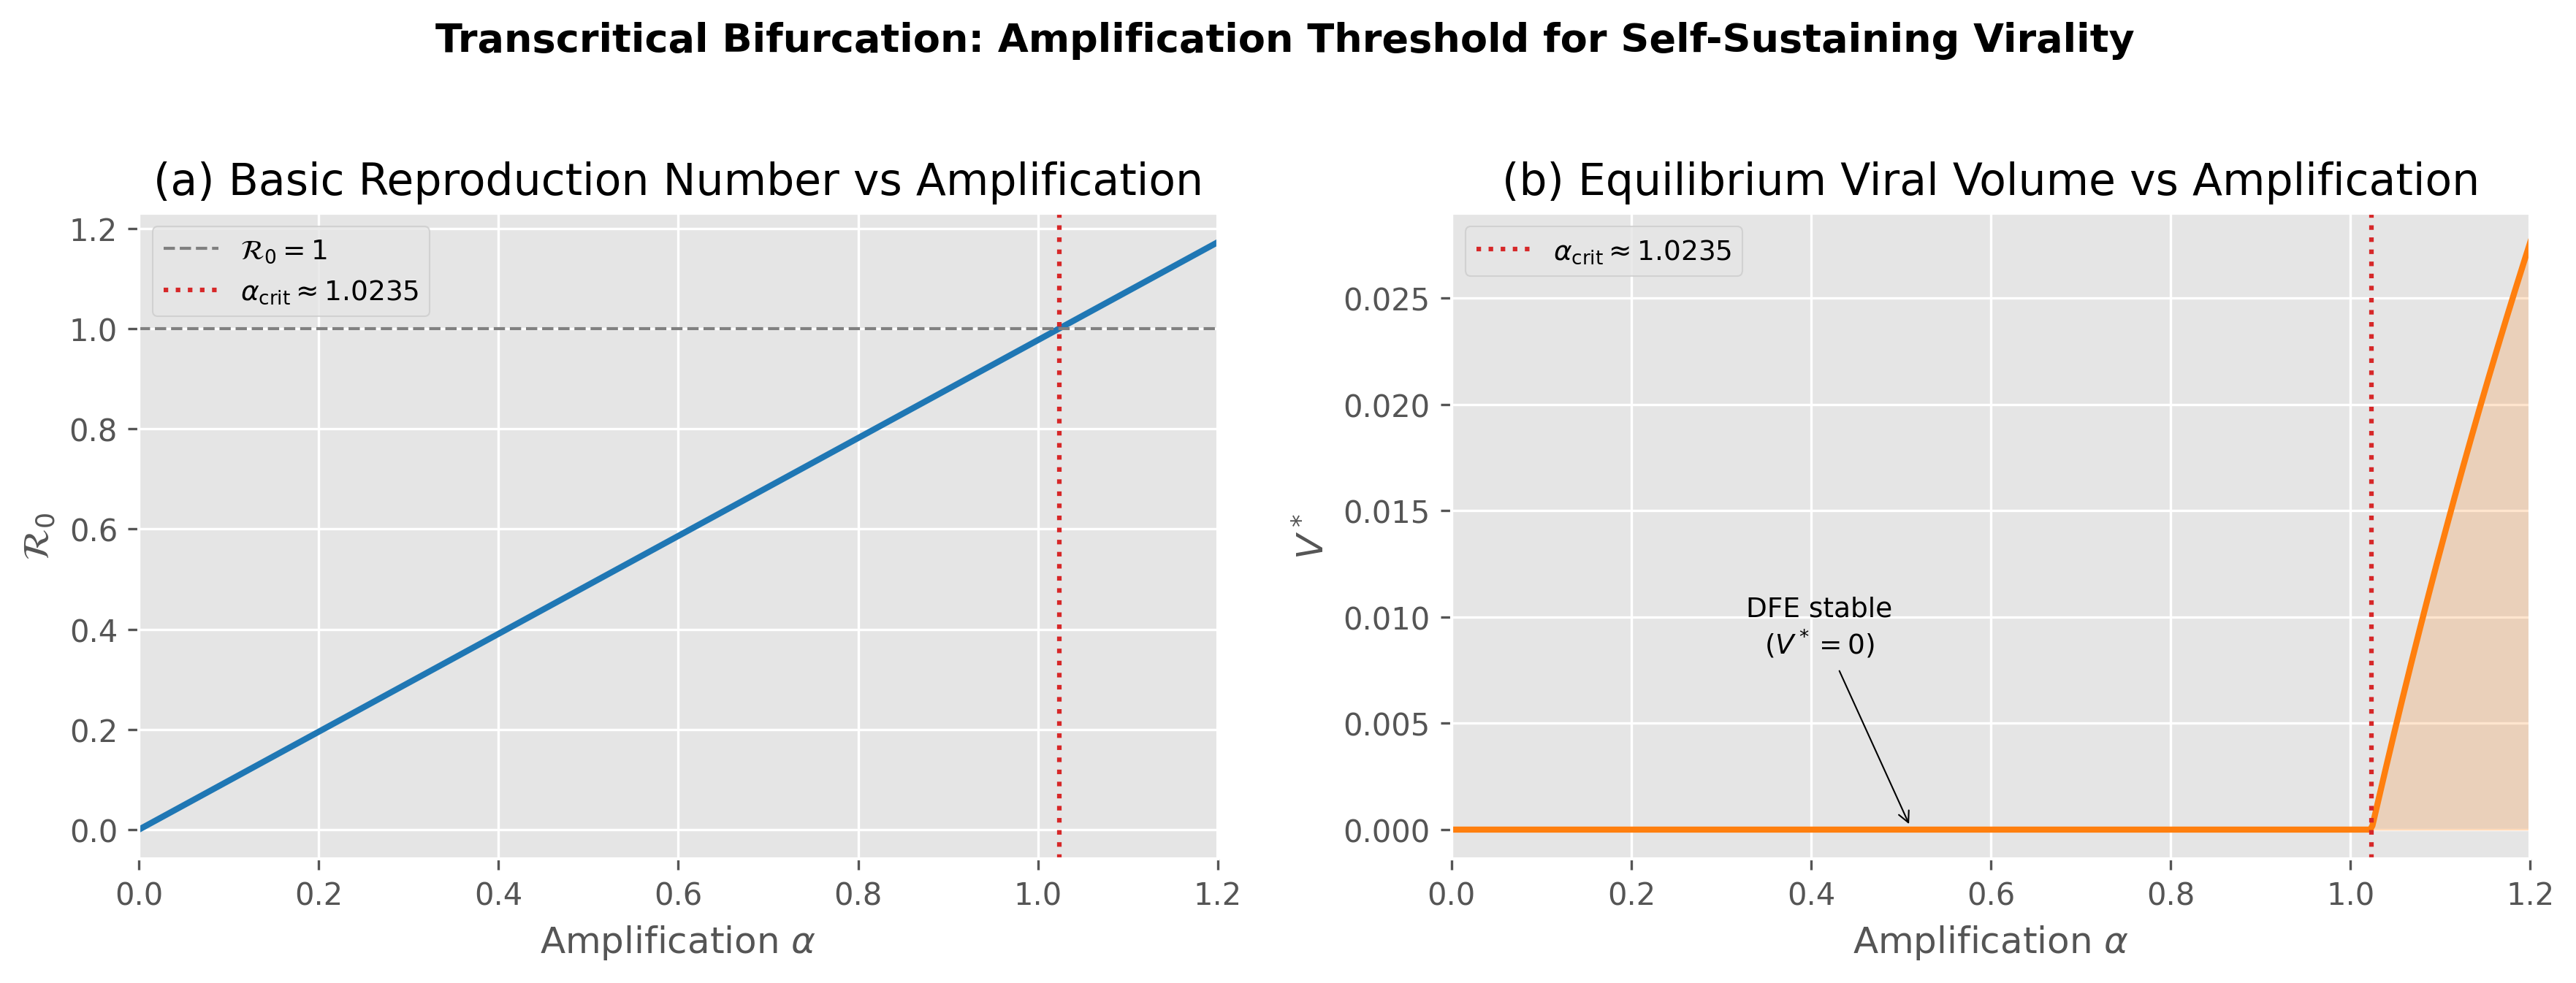
\includegraphics[width=\linewidth,height=0.70\textheight,keepaspectratio]{r0_bifurcation.png}
    \end{column}
    \begin{column}{0.43\textwidth}
      \begin{alertblock}{Key numbers}
        Moderate ($\alpha\!=\!0.5$) to aggressive ($\alpha\!=\!0.9$):
        \begin{itemize}
          \item Viral volume up 73\%
          \item Discussion pressure up 73\%
          \item User base down 40\%
        \end{itemize}
      \end{alertblock}

      \vspace{0.5em}
      Sensitivity analysis: spread parameters ($\gamma_0$, $\alpha$, $\beta_0$) dominate
      viral volume; pressure parameters ($\phi$, $w$) drive user retention.
    \end{column}
  \end{columns}
\end{frame}

% ═══════════════════════════════════════════════════════════════
%  SLIDE 6: CALIBRATION AND LIMITATIONS
% ═══════════════════════════════════════════════════════════════
\begin{frame}{Calibration and Limitations}
  \begin{columns}[T]
    \begin{column}{0.48\textwidth}
      \begin{greenblock}{Spread block: well-identified}
        \begin{itemize}
          \item Higgs Twitter retweets, 100\,h window
          \item $R^2 = 0.92$, narrow bootstrap CIs
          \item Beats SIR benchmark ($R^2 = 0.69$)
        \end{itemize}
      \end{greenblock}
    \end{column}
    \begin{column}{0.48\textwidth}
      \begin{alertblock}{Pressure block: partial}
        \begin{itemize}
          \item Reply activity as proxy
          \item Anchored to external toxicity scale
          \item Qualitative ranking is robust
        \end{itemize}
      \end{alertblock}
    \end{column}
  \end{columns}

  \vspace{0.6em}
  \textbf{Limitation:} pressure parameters $(\phi, \psi)$ are not uniquely identified
  from available data. The spread calibration is strong; the pressure block is
  proxy-grounded.
\end{frame}

% ═══════════════════════════════════════════════════════════════
%  SLIDE 7: TAKEAWAYS
% ═══════════════════════════════════════════════════════════════
\begin{frame}{Takeaways}
  \begin{enumerate}
    \item \textbf{Threshold.} A sharp amplification threshold exists
    ($\alpha_{\mathrm{crit}} \approx 0.32$). Below it, no sustained virality.

    \vspace{0.4em}
    \item \textbf{Feedback loop.} Above threshold, a self-reinforcing cycle:
    viral content $\to$ pressure $\to$ amplified spread $\to$ more viral content.

    \vspace{0.4em}
    \item \textbf{Tradeoff.} Aggressive amplification buys engagement today at the
    cost of a smaller, more toxic, less sustainable platform tomorrow.
  \end{enumerate}

  \vspace{0.8em}
  \centering
  {\Large Thank you. \quad Questions?}

  \vspace{0.4em}
  {\small Code and report: \texttt{github.com/n33levo/apm348\_project}}
\end{frame}

% ═══════════════════════════════════════════════════════════════
%  BACKUP SLIDES (for Q&A)
% ═══════════════════════════════════════════════════════════════
\appendix

\begin{frame}{Backup: Full ODE System}
  \small
  \begin{align*}
    \dot I &= \frac{\rho\, U}{1+U} - \beta_{\mathrm{eff}}\,I\,V - (\delta + \mu_c)\,I \\[3pt]
    \dot V &= \beta_{\mathrm{eff}}\,I\,V - \gamma_{\mathrm{eff}}\,V - \mu_c\,V \\[3pt]
    \dot F &= \gamma_{\mathrm{eff}}\,V - \mu_c\,F \\[3pt]
    \dot S &= \delta\,I - \mu_c\,S \\[3pt]
    \dot \tau &= \phi\,V - \psi\,\tau \\[3pt]
    \dot U &= \nu - \lambda_u(1+w\tau)\,U
  \end{align*}
  \[
  \beta_{\mathrm{eff}} = \alpha\,\beta_0\,(1+\kappa\,\tau), \qquad
  \gamma_{\mathrm{eff}} = \gamma_0\,(1+\eta\,\tau)
  \]
\end{frame}

\begin{frame}{Backup: Scenario Numbers \& Sensitivity}
  \small
  \centering
  \begin{tabular}{lccccc}
    \toprule
    Scenario & $\alpha$ & $\mathcal R_0$ & $V^*$ & $\tau^*$ & $U^*$ \\
    \midrule
    Engagement-first & $0.9$ & $2.84$ & $0.1203$ & $0.0674$ & $29.88$ \\
    Moderate          & $0.5$ & $1.58$ & $0.0697$ & $0.0390$ & $35.97$ \\
    Health-first      & $0.2$ & $0.63$ & $0.0000$ & $0.0000$ & $50.00$ \\
    \bottomrule
  \end{tabular}

  \vspace{0.6em}
  \begin{tabular}{lccc}
    \toprule
    & $S(V^*,p)$ & $S(\tau^*,p)$ & $S(U^*,p)$ \\
    \midrule
    $\alpha$   & $+1.67$ & $+1.67$ & $-0.47$ \\
    $\beta_0$  & $+1.67$ & $+1.67$ & $-0.47$ \\
    $\gamma_0$ & $-2.59$ & $-2.59$ & $+0.73$ \\
    $\phi$     & $\approx 0$ & $+1.00$ & $-0.28$ \\
    $\psi$     & $\approx 0$ & $-1.00$ & $+0.28$ \\
    \bottomrule
  \end{tabular}
\end{frame}

\begin{frame}{Backup: Pressure Configurations}
  \small
  \centering
  \begin{tabular}{lcccc}
    \toprule
    Configuration & $\phi$ & $\psi$ & Proxy $R^2$ & Moderate $\tau^*$ \\
    \midrule
    Current baseline & $0.056$ & $0.100$ & $0.18$ & $0.039$ \\
    Higgs decay-anchored & $0.061$ & $0.041$ & $0.10$ & $0.104$ \\
    External scale & $0.146$ & $0.100$ & $0.31$ & $0.102$ \\
    Reference-constrained & $0.417$ & $0.286$ & $0.41$ & $0.102$ \\
    Higgs unconstrained & $0.960$ & $1.000$ & $0.74$ & $0.067$ \\
    \bottomrule
  \end{tabular}

  \vspace{0.6em}
  \small
  The qualitative policy ranking (engagement-first $>$ moderate $>$ health-first for pressure) is preserved across \textbf{all five} configurations.
\end{frame}

\begin{frame}{Backup: Well-Posedness}
  \small
  \begin{itemize}
    \item \textbf{Nonnegativity:} Every face of $\mathbb{R}^6_{\geq 0}$ is inward-pointing.
    \item \textbf{Boundedness:} $U \leq \nu/\lambda_u$, total content $C \leq \rho/\mu_c$, $\tau \leq \phi C_{\max}/\psi$.
    \item \textbf{DFE stability:} Jacobian has block-triangular structure; $V$-eigenvalue is $(\gamma_0+\mu_c)(\mathcal{R}_0-1)$.
    \item \textbf{Positive equilibrium:} Numerically verified LAS at all tested $\alpha > \alpha_{\mathrm{crit}}$.
  \end{itemize}
\end{frame}

\begin{frame}{Backup: Higgs Dataset Overview}
  \centering
  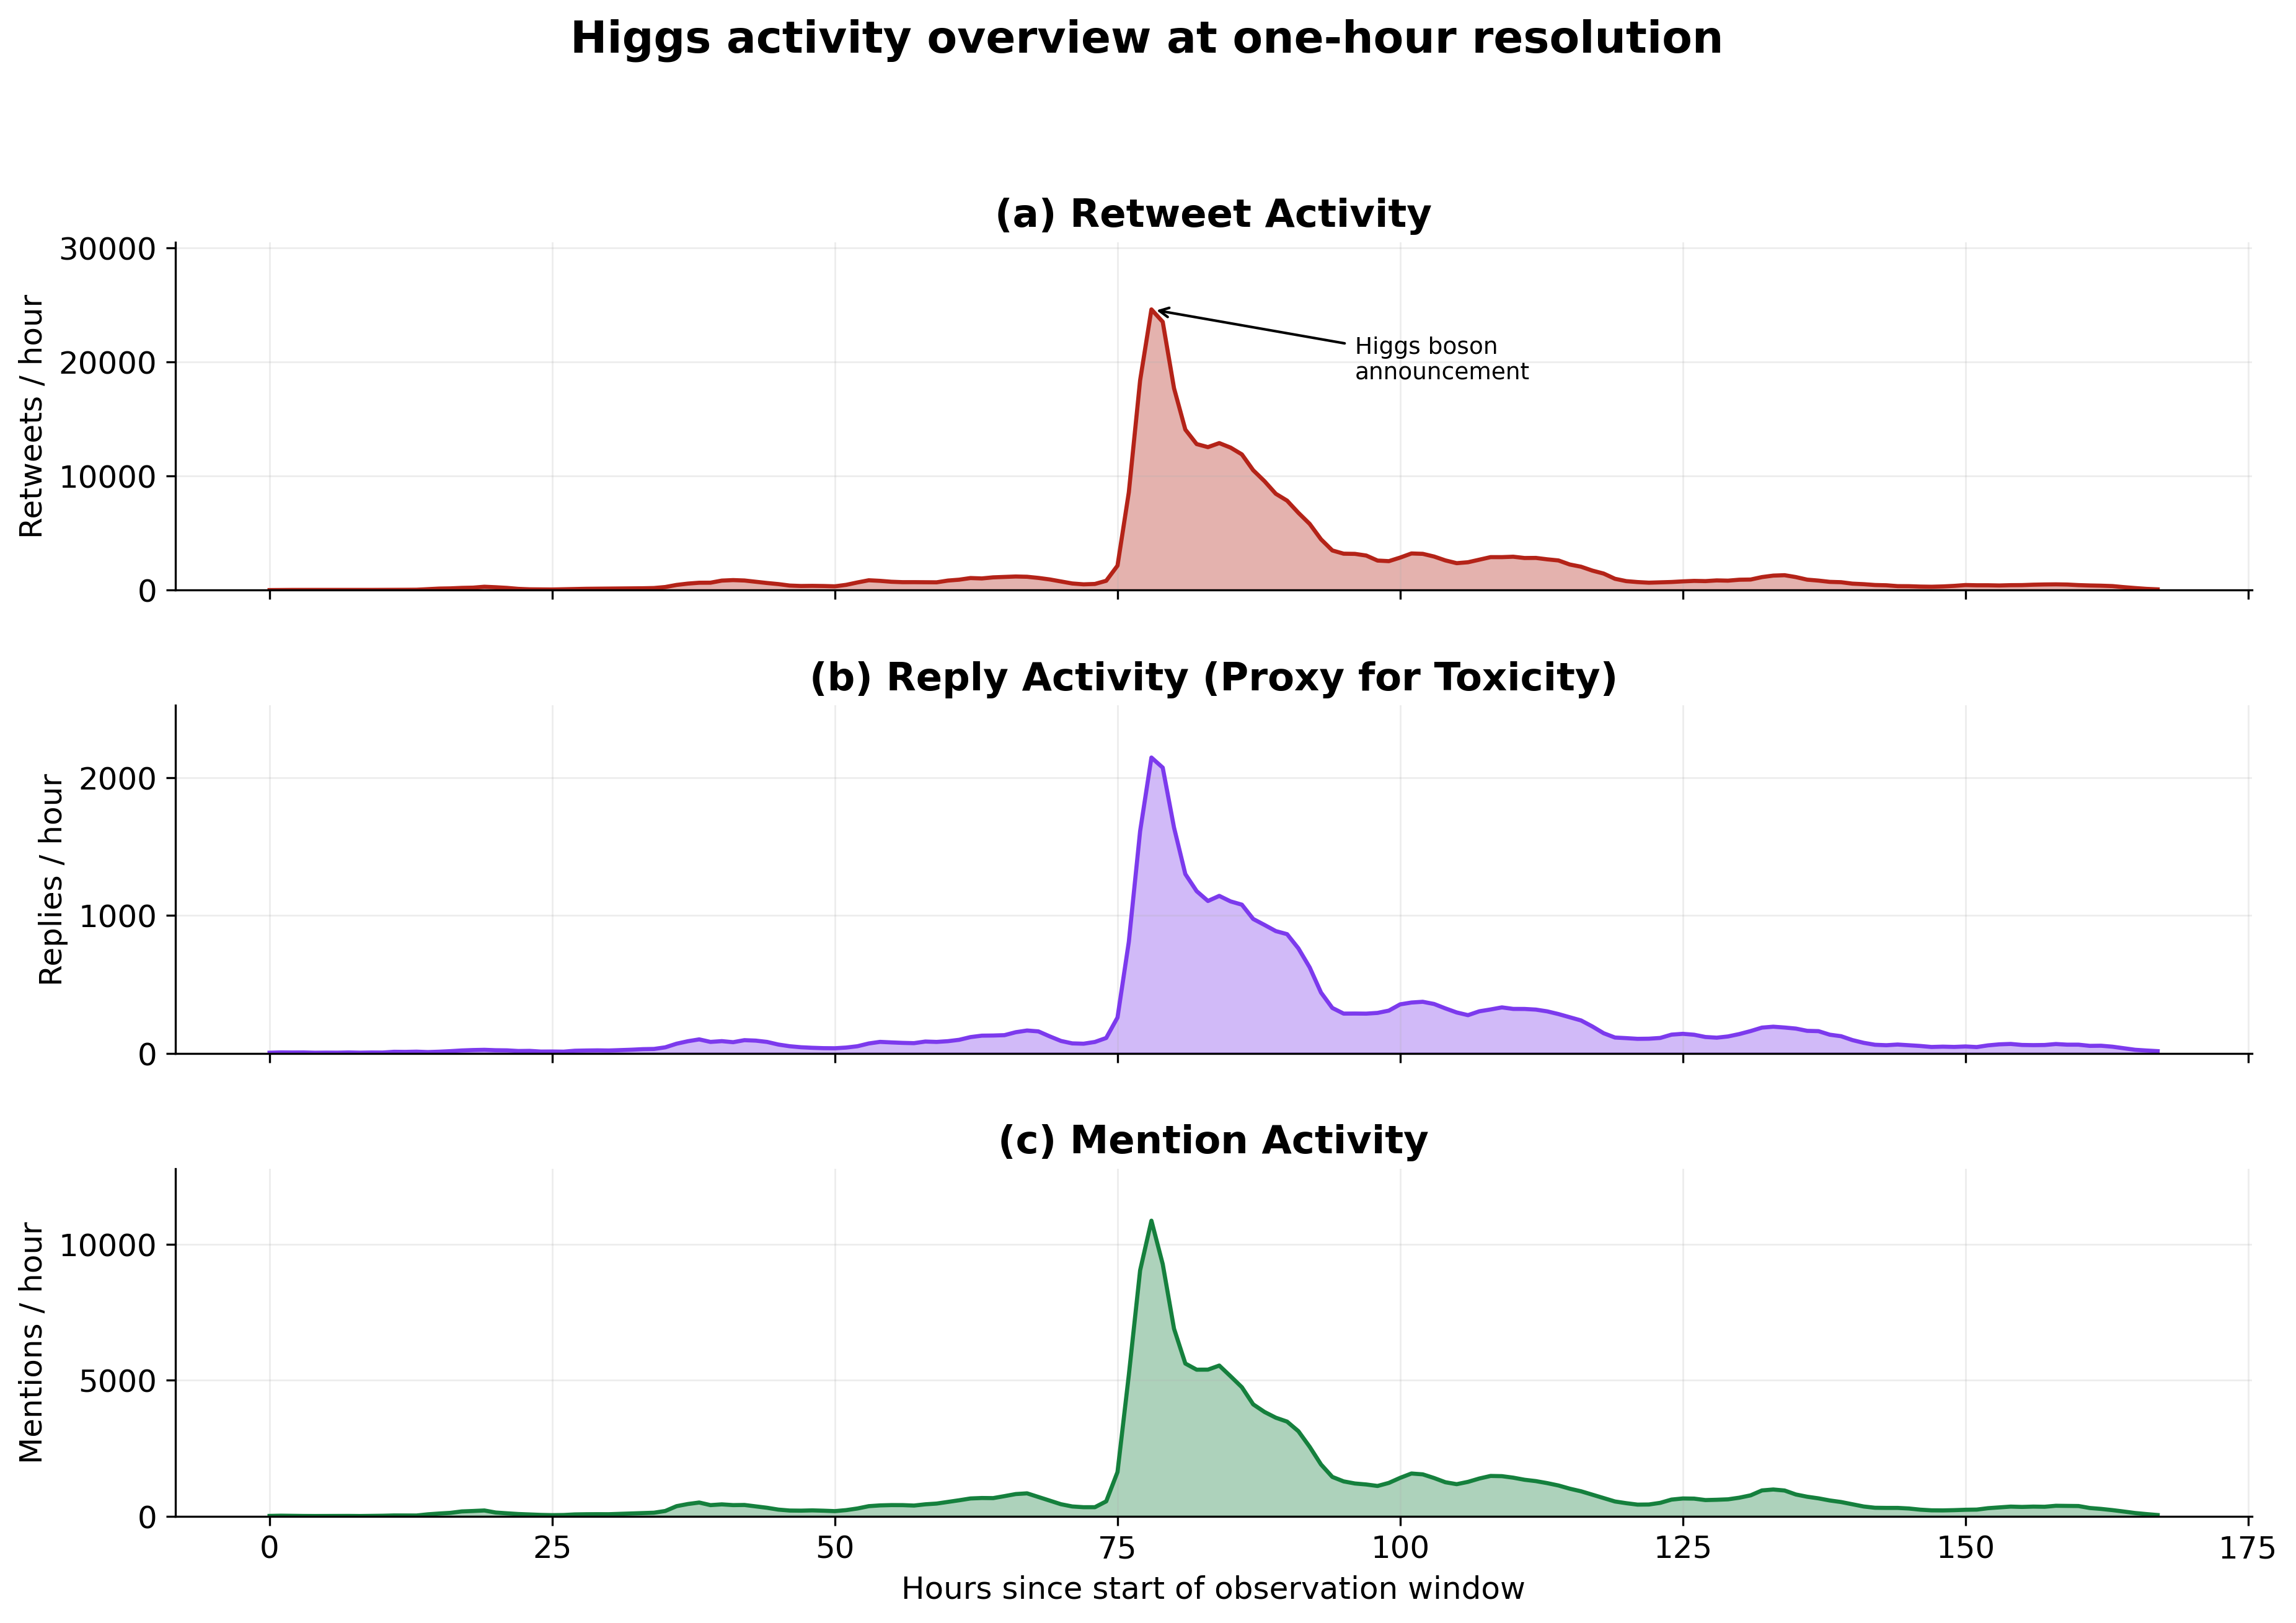
\includegraphics[width=0.85\linewidth,height=0.75\textheight,keepaspectratio]{higgs_overview.png}
\end{frame}

\begin{frame}{Backup: $\phi$ Sensitivity}
  \centering
  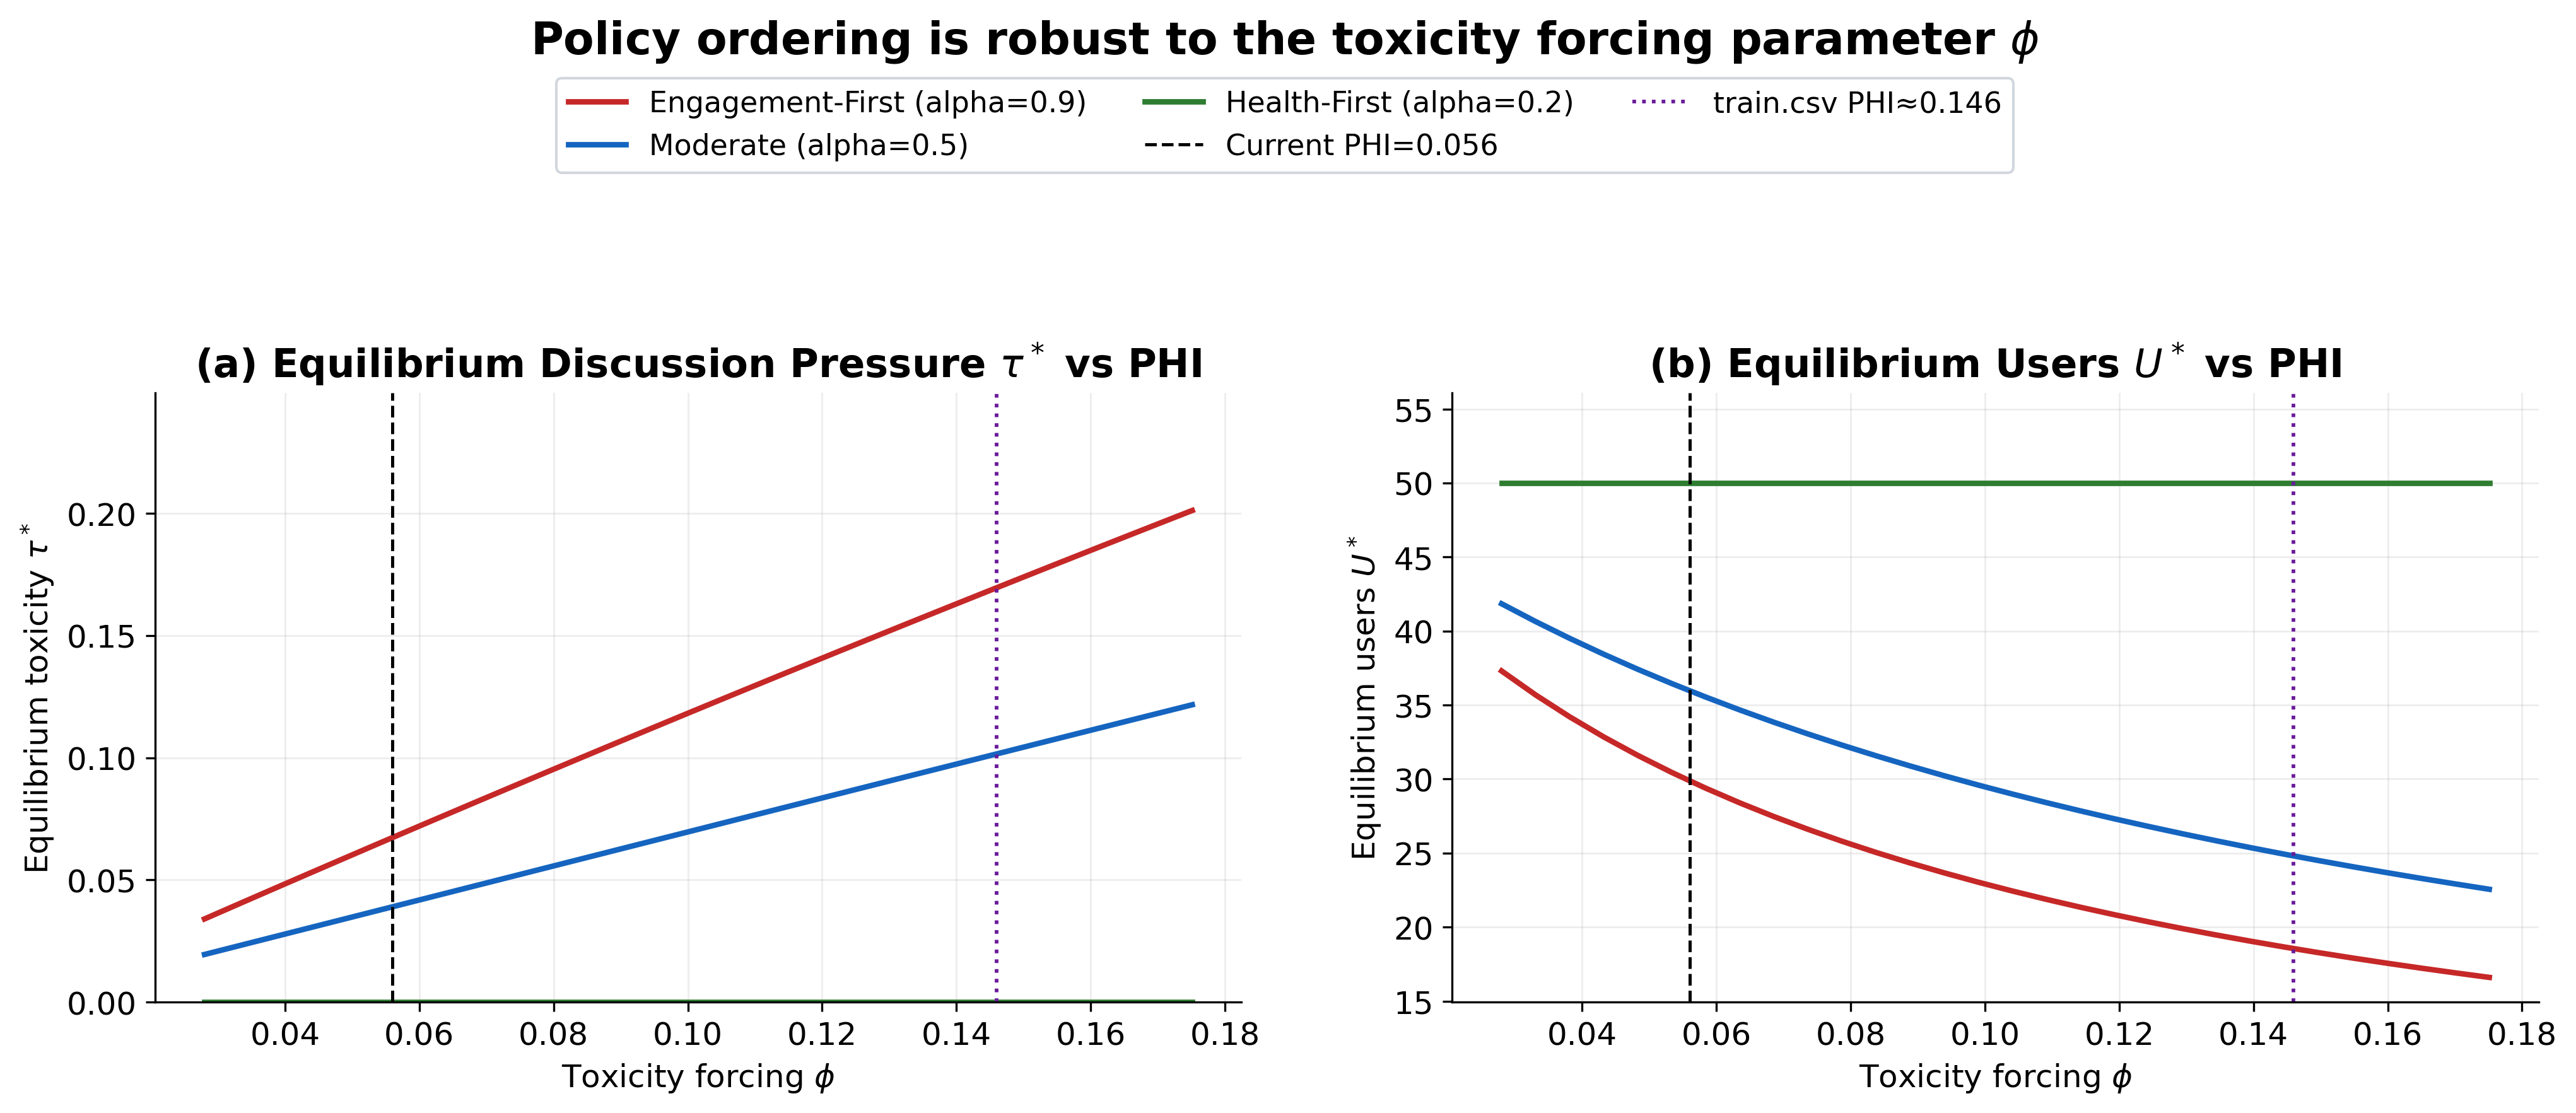
\includegraphics[width=0.85\linewidth,height=0.75\textheight,keepaspectratio]{phi_sensitivity.png}
\end{frame}

\end{document}
